\documentclass[a4paper,12pt]{article}
\usepackage{blindtext}
\usepackage[utf8]{inputenc}
\usepackage{graphicx}
\usepackage{enumitem}
\usepackage{booktabs}
\usepackage{verbatim}
\usepackage{makecell}
\usepackage[section]{placeins}
\usepackage{float}

\begin{document}
\begin{titlepage}
\center


\textsc{\LARGE Department of Computer Science} \\ [.5cm]
\textsc{\Large Project: NavUP} \\ [.5cm]
\textsc{\Large Client: Department of Computer Science, University of Pretoria} \\ [.5cm]
\line(1,0){450}\\[.5cm]
\huge{\bfseries Software Requirement Specification}\\
\line(1,0){450}\\[.5cm]
\textsc{\LARGE Team Jelly}\\ [0.5cm]

\begin{minipage}{0.4\textwidth}
\begin{flushleft} \large
\textbf{Author(s):}\\
Mpho \textsc{Baloyi}\\
Seonin  \textsc{David}\\
Cian  \textsc{Steenkamp}\\
Victor \textsc{Twigge}\\
Wanrick  \textsc{Willemse}\\
Idrian  \textsc{van der Westhuizen}\\
\end{flushleft}
\end{minipage}
~
\begin{minipage}{0.4\textwidth}
\begin{flushright} \large
\textbf{Student number(s):} \\
14133670\\
15063021\\
15095682\\
10376802\\
29560617\\
15078729\\
\end{flushright}
\end{minipage}\\


\vfil

\end{titlepage}
\newpage
\tableofcontents
\newpage

\newpage
\section{Introduction}
This section provides an outline of this Software Requirements Specification(SRS). The purpose for this document and the scope it covers is described and a definition list is provided for abbreviations.
\subsection{Purpose}
The purpose of this Software Requirements Specification(SRS) is to describe the requirements and specifications of the NavUP system,a mobile navigation application for the University of Pretoria, Hatfield campus. It contains details about the functional features of the NavUP system,along with the interface details,design constraints and related considerations such as software quality attributes. \\
Further specific requirements are detailed within the document and makes mention of functional requirements and other constraints to give a finer detail of what is expected in the NavUP system. This SRS documents is intended for the clientèle that will oversee the development of the NavUP system.
\subsection{Scope}
The 'NavUP' system will be used to navigate around the University of Pretoria Hatfield campus. The software will include a map of the campus that distinguishes between food courts, lecture halls, administrative buildings and other locations of interests.\\
The system will allow a user to identify his current location on campus and search for a destination on campus. The system will then determine the ideal route to the destination based on restrictions specified by the user such as avoiding pedestrian traffic
and provide directions. Heat maps will then be used to reveal congested areas and show where large number of students are moving in close proximity. The system will also provide users with information about activities and events that are taking place on campus as well information about points of interests.  
The system will also include game-like functionality that will award badges to users who have achieved certain distance milestones, and to those who travel to a new area for the first time.\\
The software will run on any Android or iOS smart phone or tablet. The system will mainly use WiFi connectivity to determine users' locations.
\subsection{Definitions, Acronyms and Abbreviations}
SRS:	Software Specifications Requirement\\
UP:		University of Pretoria\\
GPS:	Global Positioning System \\
Admin:  Administration
\subsection{References}
 Kung, D. (2014). Object-oriented software engineering. 1st ed. McGraw-Hill, p.98.
\subsection{Overview}
The SRS firstly gives an overall description of the NavUP system and its various interfaces. Each interface is divided into a separate subsection where further detail is given about what it must do and how it interacts with other interfaces. Afterwards the SRS makes mention of the memory constraints and operations. The requirements to the site adaptation are specified further in the SRS documentation.\\
The SRS describes the average expected user for NavUP the system and what constraints the developers need to take into account when designing the overall system in more detail. A list of assumptions and dependencies of the user and the overall system is given that were used to design the basic functionality of the NavUP system detailed in the SRS document.\\
Specific requirements are given for the external interface and functional requirements. The functional requirements contains smaller logical modules and how they might work. Performance requirements that describes how the NavUP system should perform and what is expected of its performance along with design constraints are given for the NavUP system. The SRS then describes the various quality attributes the system should have in order to function reliably.
\section{Overall Description}
\subsection{Product Perspective}
\subsubsection{System interfaces}
The system is going to be designed in a modular fashion, where the separate functionalities are broken up to allow for multiple programmers and designers to work on the NavUP at once. The modularity also allows for better maintenance and upgrading of future software and/or hardware by allowing the programmers to only change a smaller group of modules.\\
The System will need to be coded in such a way that multiple types of mobile devices would be able to use the NavUP system. It must also be able to communicate with an external database/server such as ClickUP where user information can be tracked and saved for further use in other applications and functionalities.
\subsubsection{User interfaces}
The user interface should be designed for a mobile device, in other words the screen should not be cluttered with icons and make use of touch screen technologies and its gestures. The map of the Hatfield campus along with various points of interest should be clearly visible on the screen. The user interface must be unambiguous since not only students and staff will make use of the NavUP system, but visitors as well. Since visitors will make use of the system, a way to locate and find various building by name would be beneficial, not only for visitors, but perhaps first year students as well.
\subsubsection{Hardware interfaces}
The NavUP system should be able to make use of the Wi-Fi routers scattered throughout the Hatfield campus. The application itself should be able to run on a mobile device and therefore make use of phone data alongside the Wi-fi routers and make use of the built-in GPS system on most mobile devices. The NavUP application should be able to support input from touch screen devices from the user’s mobile device to communicate and request various functionalities of the system.\\
The system should also make use of an external database to track a user’s progress for various achievement based activities. The system would also be able to use the database to direct specific help/information to the user.
\subsubsection{Software interfaces}
The various classes and modules programmed on the software of the system should be capable of receiving data from the hardware and communications functions of the system. The software should be able to calculate and update values on the internal system as well as the external database. Various classes and modules should be able to send and receive values from one another and these updated/received values should be able to communicate with the mobiles devices interface in order to update the map. The software should also be capable of updating the data of the external database.\\
\subsubsection{Communication Interfaces}
The mobile device used by the user should be able to communicate with the Wi-Fi routers throughout the Hatfield campus in order to update values such as coordinates on the system. The user’s mobile device should also be able to send and receive data from an external database, this data can also be used to block/allow access to certain features for instance a student must be able to participate in game like activities, but a visitor does not have to. Various mobile devices should be able to communicate with their navigation systems and other mobile devices (directly or indirectly) in order to calculate and create heat maps of high user traffic in an area on the map.
\subsubsection{Memory}
Because this application will be mainly mobile based, it should use as little as possible primary memory. It must in no way overload the mobile device's functional capacity. The installation size must be small, to not clutter up user space on the user's device. Application download should also preferably take place over the UP WiFi network to alleviate user data costs.\\
The entire system will also make use of an external database in order to save and track user progress and various other events, this way the user need only retrieve the data from the external database rather than waste the memory space of the mobile device.
\subsubsection{Operations}
\subsubsection{Site Adaptation Requirements}
\subsection{Product Functions}
\subsection{User Characteristics}
The following is a list of the four types of users for the NavUP system and the different ways in which
they interact with the system.
\begin{itemize} 
	\item[$\bullet$] Students
	\begin{itemize}  
	\item This group of users will use the front-end of the system, which consists of a mobile application which will run
	on various mobile devices.
	\item Students will be provided with ability to view their current location, search and locate venues and navigate to       			destinations without the need to log in.
	\item To enjoy the benefits of saving locations, receive personalized information such as activities and events based on 		       points of interest, students need to be logged in.
	 \end{itemize}
	\item[$\bullet$] University Of Pretoria Staff 
	\begin{itemize}
	\item This group of users will use both the front-end and back-end of the system,they will use the back-end 
	to add view and change user details. 
	\item The front-end may be used the same way it is used by students. 
	\end{itemize}  
	\item[$\bullet$] Guests  
	\begin{itemize}  
	\item Guest users will be able to view their location, search venues, view events and navigate to destinations. 
	\end{itemize}
	\item[$\bullet$] Administrators of the NavUP system 
	\begin{itemize}  
	\item This group of users will use the back-end part of the system. 
	\item They will be able to add, remove and manage the following: users, activities and event notifications.
	\item They are responsible for the running of the system. 
	\end{itemize}
\end{itemize}

\subsection{Constraints}
The mobile application is constrained by the system interface to the WiFi hardware within the mobile phone. Since there are multiple WiFi manufacturers, the interface will most likely not be the same for every one of them. Also, there may be a difference in the performance and specifications of the hardware. \\
The Internet connection is also a constraint for the application. Since the application fetches data from the database over the Internet, it is crucial that there is an Internet connection for the application to function. 
Both the back-end and the mobile application will be constrained by the capacity of the database. 

\subsection{Assumption and Dependencies}
An assumption about the product is that it will always be used on mobile phones that have built-in WiFi hardware and have enough performance to run the application in a working and consistent manner.
Another assumption is that the WiFi components in all mobile phones work in the same way. If the phones have different interfaces to the WiFi, the application need to be specifically adjusted to each interface and that would mean the integration with the WiFi would have different requirements than what is stated in this specification. 
For the application to launch and run it will depend on a compatible operating system and version of the mobile phone.

\section{Specific Requirements}
\subsection{External Interface Requirements}
\subsubsection{User Interface}
The mobile application will interface with the supported input and output features of the host's operating system. Inputs include text that the user will enter for login or searching a venue. Outputs include the type of fonts to display text or graphics to show images or draw the map.
\subsubsection{Hardware Interfaces}
Since neither the mobile application nor the web portal have any designated hardware, it does not have any direct hardware interfaces. The WiFi software in the mobile phone manages the built-in WiFi and the hardware connection to the database server is managed by the underlying operating system on the mobile phone and the web server. 
\subsubsection{Software Interfaces}
The mobile application communicates with the WiFi software in order to get signal strength information from multiple WiFi access points to determine (using triangulation) where the user is located. The communication software between the database and mobile application consists of operation concerning creating, reading, removing and modifying the data.
\subsubsection{Communication Interfaces}
The communication between the different parts of the system is important since they depend on each other. However, in what way the communication is achieved is not important for the system and is therefore handled by the underlying operating systems for both the mobile application and the back-end of the system.
\subsection{Functional Requirements}
\subsubsection{1-Admin system}
\paragraph{1-1}
The admin system will allow a designated administrator to add, remove and manage user accounts.\\
Preconditions:
\begin{itemize} 
	\item[$\bullet$] Must have admin privileges
	\item[$\bullet$] Must be registered and logged in
\end{itemize}
Postconditions:
\begin{itemize}
	\item[$\bullet$] Changes made to user accounts
\end{itemize}
\paragraph{1-2}
The admin system will allow a designated administrator to add, remove and manage system, activity and event notifications.\\
Preconditions:
\begin{itemize}
	\item[$\bullet$] Must have admin privileges
	\item[$\bullet$] Must be registered and logged in
\end{itemize}
Postconditions:
\begin{itemize}
	\item[$\bullet$] Changes made to event notifications
\end{itemize}
\begin{figure}[H]
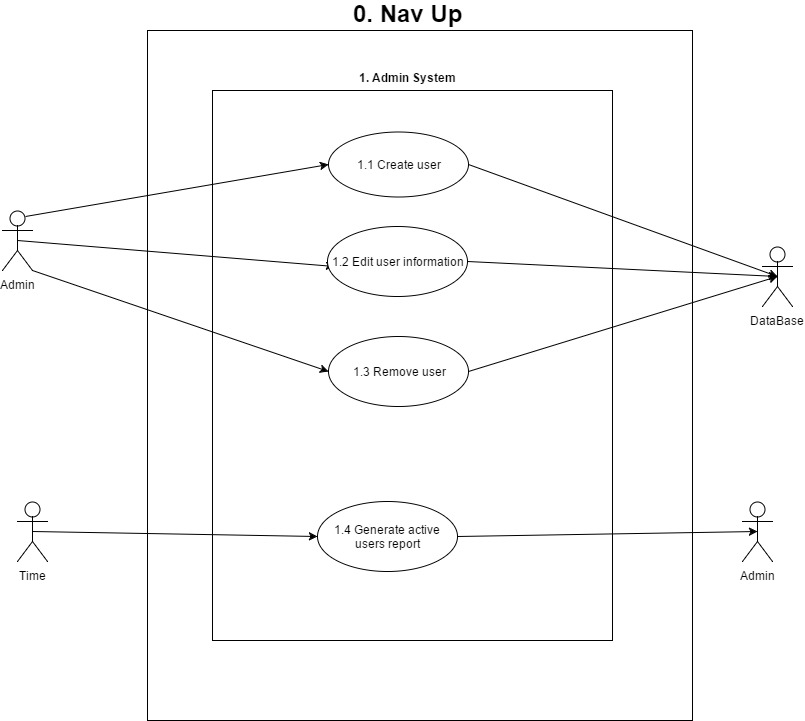
\includegraphics[width=\textwidth]{UseCaseDiagrams/AdminUCD.JPG}
\caption{Admin System use case diagram}
\label{fig:Admin Use Case Diagram}
\end{figure}
\begin{figure}[H]
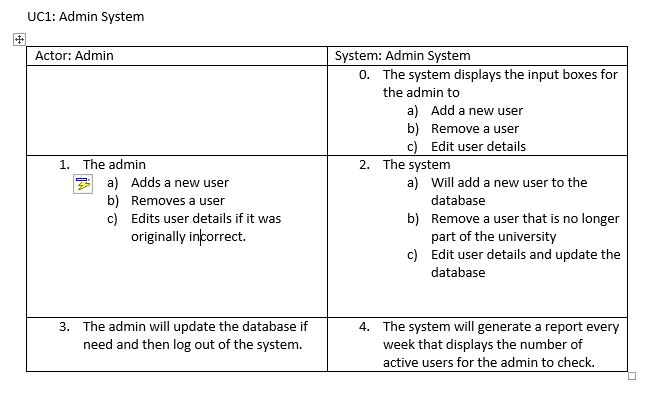
\includegraphics[width=\textwidth]{ActorDiagrams/AdminAD.JPG}
\caption{Admin System Actor Diagram}
\label{fig:Admin Actor Diagram}
\end{figure}


\subsubsection{2-Account management}
\paragraph{2-1}
The account management system will allow a registered user (staff member and student) to login to the system.\\
Preconditions:
\begin{itemize}
	\item[$\bullet$] Must be registered
\end{itemize}
Postconditions:
\begin{itemize}
	\item[$\bullet$] User logged in
\end{itemize}
\paragraph{2-2}
The account management system will allow a guest user to login to the system using a guest account.\\
Preconditions:
\begin{itemize}
	\item[$\bullet$] Must be a visitor
\end{itemize}
Postconditions:
\begin{itemize}
	\item[$\bullet$] User logged in
\end{itemize}
\paragraph{2-3}
The account management system will allow a registered user (staff member and student) to view and change user details.\\
Preconditions:
\begin{itemize}
	\item[$\bullet$] Must be registered and logged in
\end{itemize}
Postconditions:
\begin{itemize}
	\item[$\bullet$] Changes made to user details
\end{itemize}
\paragraph{2-4}
The account management system will allow an administrator to make a change to the account system, ie what details about users are stored.\\
Preconditions:
\begin{itemize}
	\item[$\bullet$] Must have admin privileges
	\item[$\bullet$] Must be registered
\end{itemize}
Postconditions:
\begin{itemize}
	\item[$\bullet$] Changes made to account management system
\end{itemize}
\begin{figure}[H]
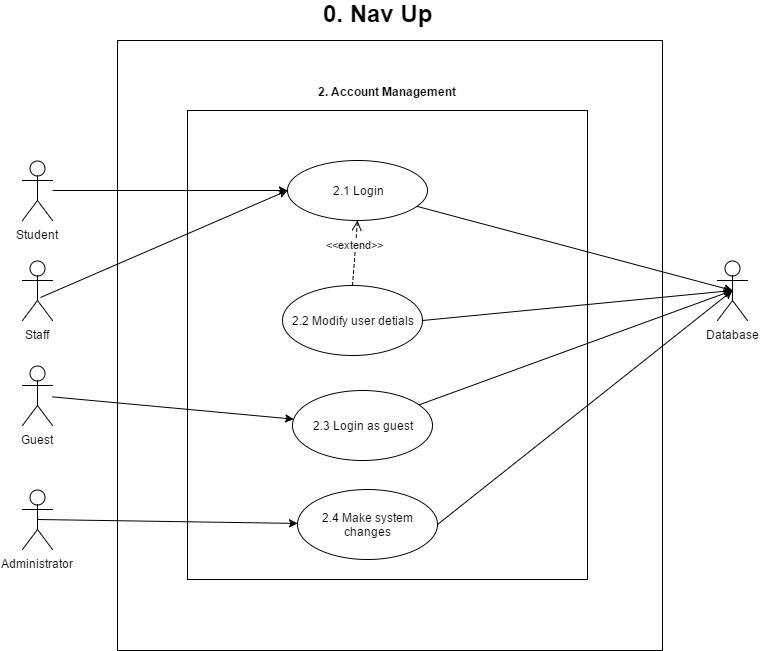
\includegraphics[width=\textwidth]{UseCaseDiagrams/AccManagementUCD.JPG}
\caption{Account Management use case diagram}
\label{fig:Account Management Use Case Diagram}
\end{figure}
\begin{figure}[H]
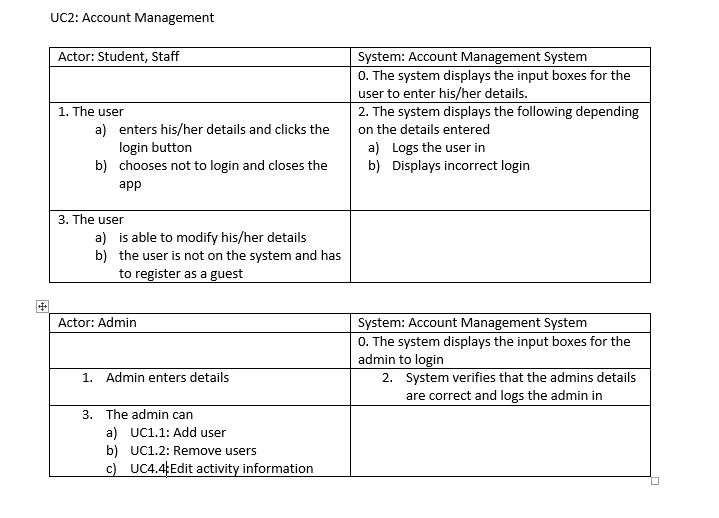
\includegraphics[width=\textwidth]{ActorDiagrams/AccManagementAD.JPG}
\caption{Account Management Actor Diagram}
\label{fig:Account Management Actor Diagram}
\end{figure}


\subsubsection{3-Core-Navigation system}

\paragraph{3-1}
The core navigation system will allow a user to view his/her current location.\\
Preconditions:
\begin{itemize}
	\item[$\bullet$] Must be registered and logged in
	\item[$\bullet$] Must be on campus and connected to WiFi network
\end{itemize}
Postconditions:
\begin{itemize}
	\item[$\bullet$] User sees his/her location
\end{itemize}
\paragraph{3-2}
The core navigation system will allow a user to save his/her current location details for later retrieval.\\
Preconditions:
\begin{itemize}
	\item[$\bullet$] Must be registered and logged in
	\item[$\bullet$] Must be on campus and connected to WiFi network
	\item[$\bullet$] Must view current location
\end{itemize}
Postconditions:
\begin{itemize}
	\item[$\bullet$] User saves his/her location
\end{itemize}
\paragraph{3-3}
The core navigation system will allow a user to enter a destination and get directions. This will utilize the heat map to find and indicate an optimal route based on pedestrian congestion.\\
Preconditions:
\begin{itemize}
	\item[$\bullet$] Must be registered and logged in
	\item[$\bullet$] Must be on campus and connected to WiFi network
\end{itemize}
Postconditions:
\begin{itemize}
	\item[$\bullet$] User sees optimal route and heat map
\end{itemize}
\begin{figure}[H]
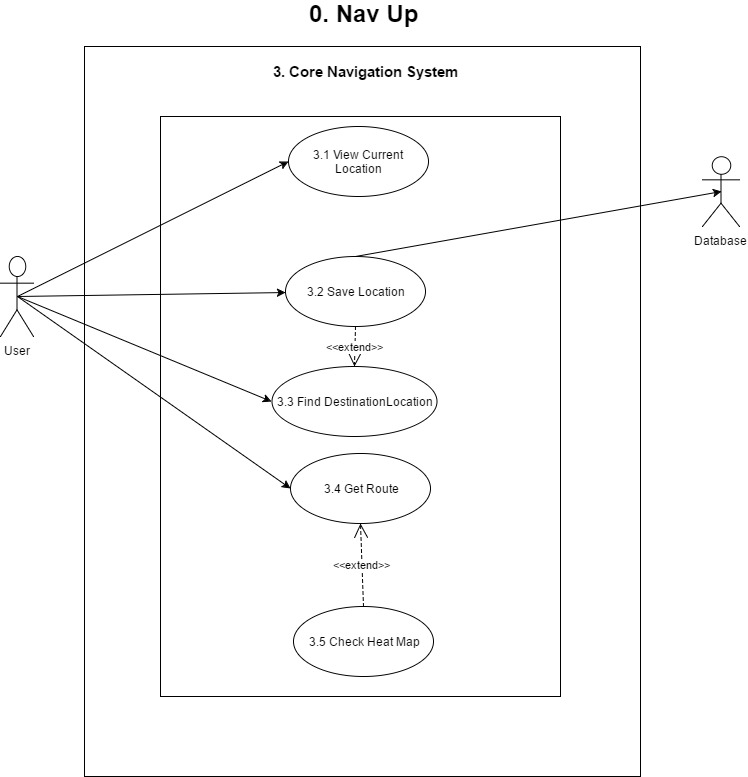
\includegraphics[width=\textwidth]{UseCaseDiagrams/CoreNavUCD.JPG}
\caption{Core Navigation use case diagram}
\label{fig:Core Navigation Use Case Diagram}
\end{figure}
\begin{figure}[H]
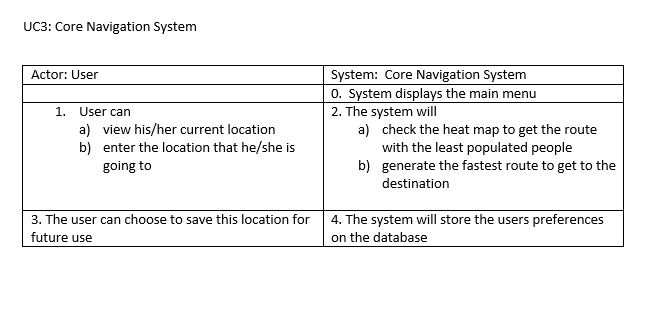
\includegraphics[width=\textwidth]{ActorDiagrams/CoreNavAD.JPG}
\caption{Core Navigation Actor Diagram}
\label{fig:Core Navigation Actor Diagram}
\end{figure}


\subsubsection{4-Activity management}

\paragraph{4-1}
The activity management system will allow a user to manage current activities.\\
Preconditions:
\begin{itemize}
	\item[$\bullet$] Must be registered and logged in
	\item[$\bullet$] Must be on campus and connected to WiFi network
\end{itemize}
Postconditions:
\begin{itemize}
	\item[$\bullet$] Changes made to activity list
\end{itemize}
\paragraph{4-2}
The activity management system will allow a user to add an activity to an activity list.\\
Preconditions:
\begin{itemize}
	\item[$\bullet$] Must be registered and logged in
	\item[$\bullet$] Must be on campus and connected to WiFi network
\end{itemize}
Postconditions:
\begin{itemize}
	\item[$\bullet$] Activity added to list
\end{itemize}
\paragraph{4-3}
The activity management system will allow a user to remove activities from an activity list.\\
Preconditions:
\begin{itemize}
	\item[$\bullet$] Must be registered and logged in
	\item[$\bullet$] Must be on campus and connected to WiFi network
\end{itemize}
Postconditions:
\begin{itemize}
	\item[$\bullet$] Activity removed from list
\end{itemize}
\paragraph{4-4}
The activity management system will allow a user to view the heat map of current pedestrian traffic on campus.\\
Preconditions:
\begin{itemize}
	\item[$\bullet$] Must be registered and logged in
	\item[$\bullet$] Must be on campus and connected to WiFi network
\end{itemize}
Postconditions:
\begin{itemize}
	\item[$\bullet$] User sees campus pedestrian traffic on heat map
\end{itemize}
\paragraph{4-5}
The activity management system will update a user on any relevant activity information.\\
Preconditions:
\begin{itemize}
	\item[$\bullet$] Must be registered and logged in
	\item[$\bullet$] Must be on campus and connected to WiFi network
\end{itemize}
Postconditions:
\begin{itemize}
	\item[$\bullet$] User receives notification
\end{itemize}
\begin{figure}[H]
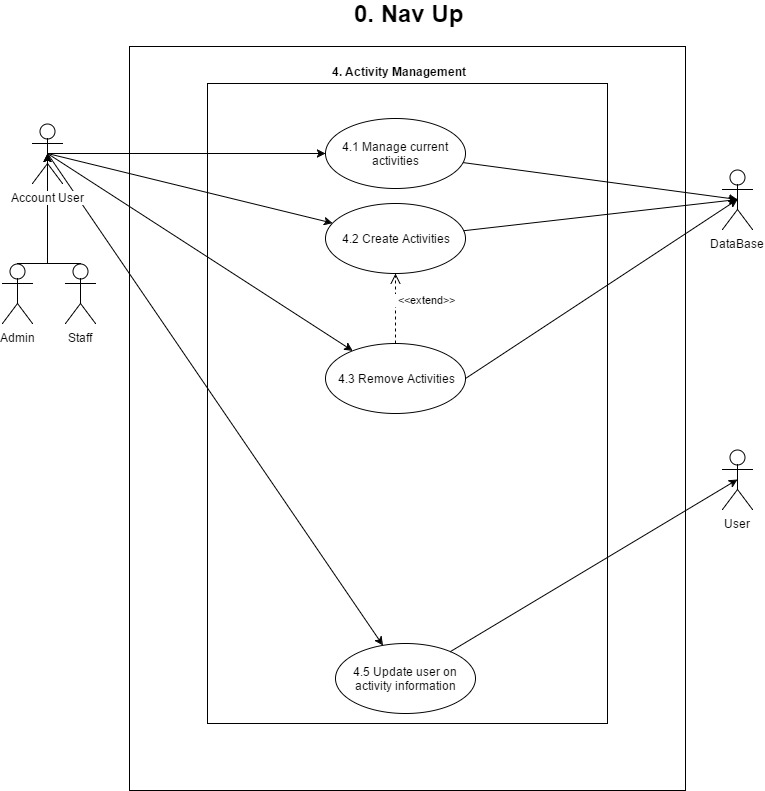
\includegraphics[width=\textwidth]{UseCaseDiagrams/ActManagementUCD.JPG}
\caption{Activity management use case diagram}
\label{fig:Activity management Use Case Diagram}
\end{figure}
\begin{figure}[H]
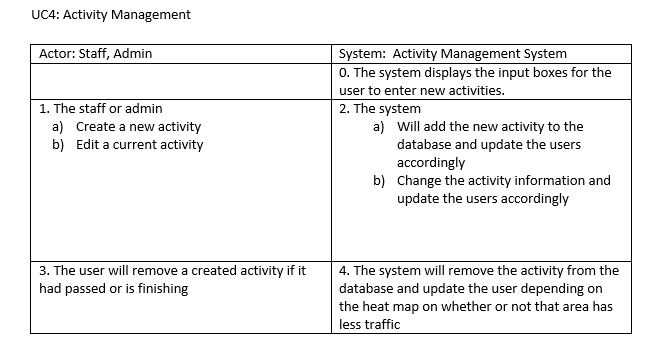
\includegraphics[width=\textwidth]{ActorDiagrams/ActManagementAD.JPG}
\caption{Activity Management System Actor Diagram}
\label{fig:Activity Management System Actor Diagram}
\end{figure}


\subsubsection{5-Notification}

\paragraph{5-1}
The notification system will allow an administrator to create a notification.\\
Preconditions:
\begin{itemize}
	\item[$\bullet$] Must be registered and logged in
	\item[$\bullet$] Must have admin privileges
\end{itemize}
Postconditions:
\begin{itemize}
	\item[$\bullet$] Notification created
\end{itemize}
\paragraph{5-2}
The notification system will allow an administrator to remove a notification.\\
Preconditions:
\begin{itemize}
	\item[$\bullet$] Must be registered and logged in
	\item[$\bullet$] Must have admin privileges
\end{itemize}
Postconditions:
\begin{itemize}
	\item[$\bullet$] Notification removed
\end{itemize}
\paragraph{5-3}
The notification system will allow an administrator to push notification to relevant users.\\
Preconditions:
\begin{itemize}
	\item[$\bullet$] Must be registered and logged in
	\item[$\bullet$] Must have admin privileges
\end{itemize}
Postconditions:
\begin{itemize}
	\item[$\bullet$] Relevant users received push notification
\end{itemize}
\begin{figure}[H]
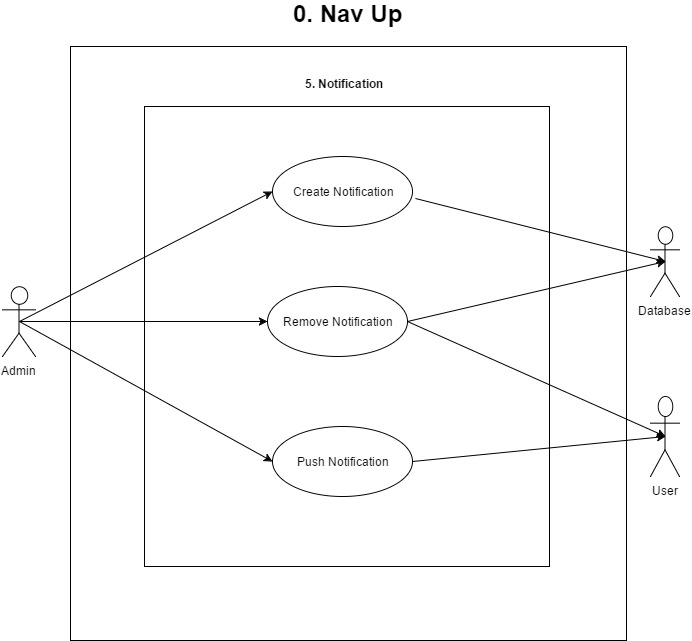
\includegraphics[width=\textwidth]{UseCaseDiagrams/NotificationUCD.JPG}
\caption{Notification use case diagram}
\label{fig:Notification Use Case Diagram}
\end{figure}
\begin{figure}[H]
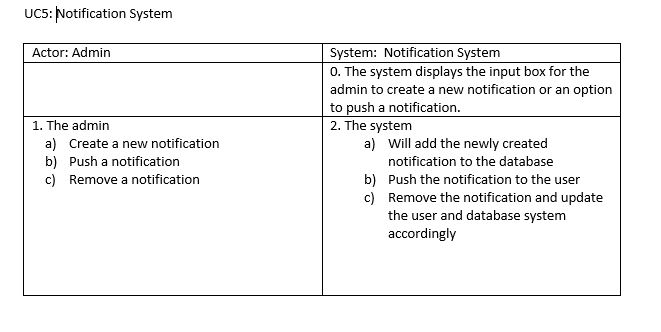
\includegraphics[width=\textwidth]{ActorDiagrams/NotificationAD.JPG}
\caption{Notification Actor Diagram}
\label{fig:Notification Actor Diagram}
\end{figure}

\subsubsection{Traceability Matrix}
\begin{figure}[H]
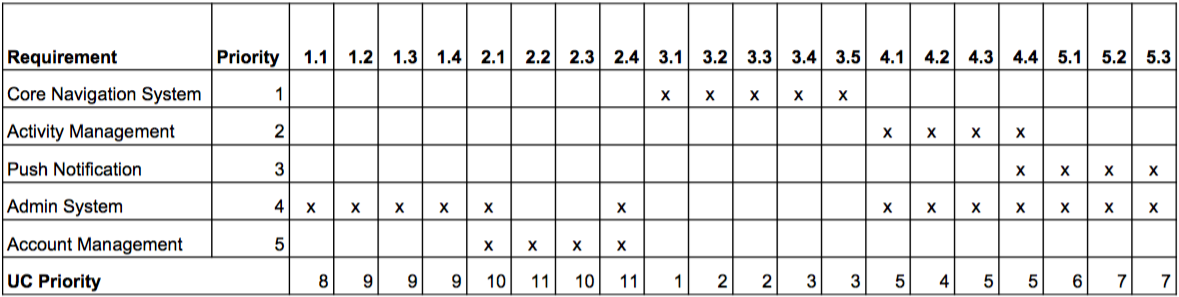
\includegraphics[width=\textwidth]{Traceability/Traceability.png}
\caption{Traceability Matrix}
\label{fig:Traceability Matrix}
\end{figure}
Use cases
\begin{itemize}
\item 1.1 Create User
\item 1.2 Edit User Information
\item 1.3 Remove User
\item 1.4 Generate Active Users Report
\end{itemize}

\begin{itemize}
\item 2.1 Login
\item 2.2 Modify user details
\item 2.3 Login as guest 
\item 2.4 Make system changes 
\end{itemize}


\begin{itemize}
\item 3.1 View Current Location
\item 3.2 Save location
\item 3.3 Find Destination 
\item 3.4 Get Route
\item 3.5 Check heat map (Determine Pedestrian Traffic)
\end{itemize}

\begin{itemize}
\item 4.1 Manage Current Activities
\item 4.2 Create Activities
\item 4.3 Remove Activities
\item 4.4 Update User Information
\end{itemize}

\begin{itemize}
\item 5.1 Create Notification
\item 5.2 Remove Notification
\item 5.3 Push Notification
\end{itemize}


\subsection{Performance Requirements}
\subsection{Design Constraints}
\subsection{Software System Attributes}
\begin{itemize}
\item[$\bullet$]Reliability:
	\begin{itemize}
		\item[$\bullet$] Any information that is stored on the database must remain correct 
		when being transferred to the user interface 
		\item[$\bullet$] The services offered by the system should be available to users except 
		for when the system is undergoing maintenance 
		\item[$\bullet$] The system should reply to user requests in the shortest time interval possible 
		\item[$\bullet$] The system must be fault tolerant,it needs to maintain a certain level of 
		performance and offer other services that are not affected by this fault to the users 
		\item[$\bullet$] In the event of a fault the system must be able to recover within the shortest
		time period possible and recover any data that may have been lost.
		\item[$\bullet$] The system should be able to respond appropriately if it receives  bad input data from the 
		user.			 
	\end{itemize}
 
\item[$\bullet$] Scalability:
	\begin{itemize}
		\item[$\bullet$] The system must be able to cater for increases in the work load, 
		for example large number of users or activities at any given time,without impacting on the 
		performance of the system.
		 \item[$\bullet$] If the system does not cater for increases in work load it should at least 
		 provide the ability to be readily enlarged/ 
	\end{itemize}
	
\item[$\bullet$] Maintainability:
	\begin{itemize}
		\item[$\bullet$] The system must be designed in a modular fashion that provides high cohesion and
		loose coupling, the will allow parts of the system to be easily maintained without affecting the rest 
		of the system.
		\item[$\bullet$] Maintenance should be able to be carried out by different maintenance teams, therefore
		the system must be easy to learn and understand.
	\end{itemize}

\item[$\bullet$] Integrability:
	\begin{itemize}
		\item[$\bullet$]Since we are following a modular design, components of the system that are
		separately developed should work  correctly together.
		\item[$\bullet$] Follow  coding standards specified by the client to allow for easy integration and employ continuous
		integration in our design process  
	\end{itemize}

\item[$\bullet$] Usability:
	\begin{itemize}
		\item[$\bullet$] The system must be easy to learn.
		\item[$\bullet$] System must cater for user mistakes,by providing the user with the undo or roll back option.
		\item[$\bullet$] The user interface must be easy to use and intuitive. 
		\item[$\bullet$] System should have options in a logical manner. 
		\item[$\bullet$] Use widgets and icons that the target users may be familiar with. 
		\item[$\bullet$] The user manual should have a detailed description of the system.
		\item[$\bullet$] A help option must be provided to the users. 
	\end{itemize}

  
\item[$\bullet$] Interoperability:
	\begin{itemize}
		\item[$\bullet$] The system must be able to communicate with the University of Pretoria WiFi system, because 
		the wifi access points will be used for the navigation.
	\end{itemize}
\end{itemize}
 
 
\subsection{Other Requirements}
	\begin{itemize} \item[$\bullet$] Low Resource Consumption \end{itemize}
		
		As mentioned above the NavUP will be running on mobile devices due to the small amount of resources some of these devices
		may have, unnecessary use of resources on the front-end of the system should be avoided.
	
\section{Appendix}
\newpage
\end{document}
